\documentclass{standalone}
\usepackage{tikz}
\usetikzlibrary{patterns, positioning}

\begin{document}
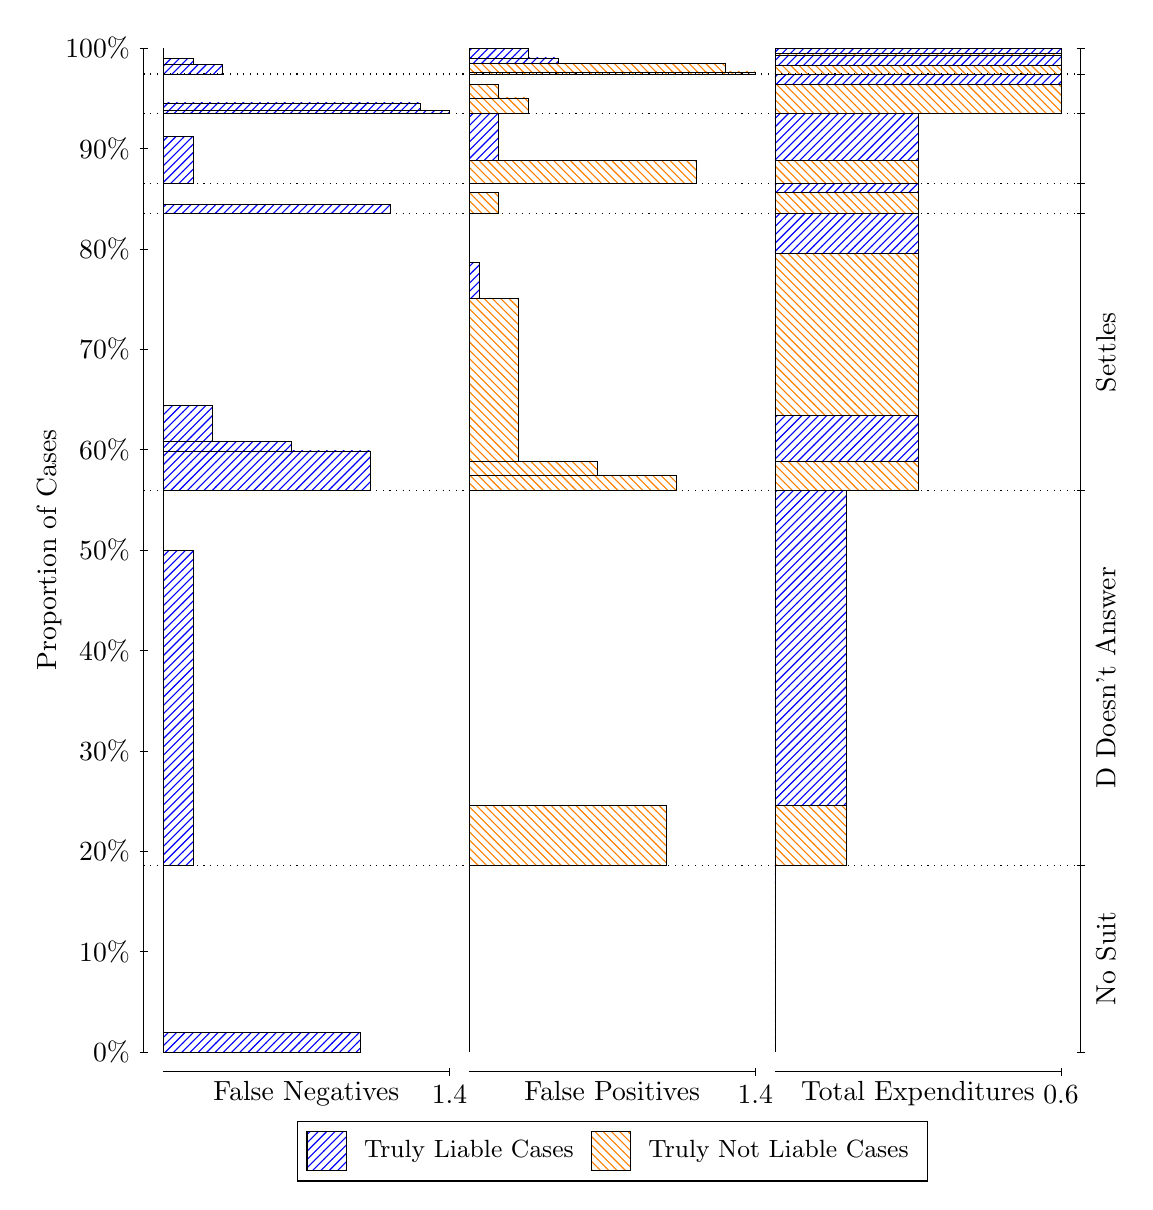
\begin{tikzpicture}
\draw[black, very thin] (1.5,1.75) -- (1.5,14.5);
\node[rotate=90, anchor=center] at (0.3, 8.125) {Proportion of Cases};
\draw[black, very thin] (1.45,1.75) -- (1.55,1.75);
\node[anchor=east] at (1.45, 1.75) {0\%};
\draw[black, very thin] (1.45,3.025) -- (1.55,3.025);
\node[anchor=east] at (1.45, 3.025) {10\%};
\draw[black, very thin] (1.45,4.3) -- (1.55,4.3);
\node[anchor=east] at (1.45, 4.3) {20\%};
\draw[black, very thin] (1.45,5.575) -- (1.55,5.575);
\node[anchor=east] at (1.45, 5.575) {30\%};
\draw[black, very thin] (1.45,6.85) -- (1.55,6.85);
\node[anchor=east] at (1.45, 6.85) {40\%};
\draw[black, very thin] (1.45,8.125) -- (1.55,8.125);
\node[anchor=east] at (1.45, 8.125) {50\%};
\draw[black, very thin] (1.45,9.4) -- (1.55,9.4);
\node[anchor=east] at (1.45, 9.4) {60\%};
\draw[black, very thin] (1.45,10.675) -- (1.55,10.675);
\node[anchor=east] at (1.45, 10.675) {70\%};
\draw[black, very thin] (1.45,11.95) -- (1.55,11.95);
\node[anchor=east] at (1.45, 11.95) {80\%};
\draw[black, very thin] (1.45,13.225) -- (1.55,13.225);
\node[anchor=east] at (1.45, 13.225) {90\%};
\draw[black, very thin] (1.45,14.5) -- (1.55,14.5);
\node[anchor=east] at (1.45, 14.5) {100\%};

\draw[black, very thin] (13.4,1.75) -- (13.4,14.5);
\draw[black, very thin] (13.35,1.75) -- (13.45,1.75);
\node[anchor=west] at (13.35, 1.75) {};
\draw[black, very thin] (13.35,4.1224) -- (13.45,4.1224);
\node[anchor=west] at (13.35, 4.1224) {};
\draw[black, very thin] (13.35,8.8791) -- (13.45,8.8791);
\node[anchor=west] at (13.35, 8.8791) {};
\draw[black, very thin] (13.35,12.397) -- (13.45,12.397);
\node[anchor=west] at (13.35, 12.397) {};
\draw[black, very thin] (13.35,12.785) -- (13.45,12.785);
\node[anchor=west] at (13.35, 12.785) {};
\draw[black, very thin] (13.35,13.668) -- (13.45,13.668);
\node[anchor=west] at (13.35, 13.668) {};
\draw[black, very thin] (13.35,14.17) -- (13.45,14.17);
\node[anchor=west] at (13.35, 14.17) {};
\draw[black, very thin] (13.35,14.5) -- (13.45,14.5);
\node[anchor=west] at (13.35, 14.5) {};

\draw[black, very thin, pattern color=blue, pattern=north east lines] (1.75,1.75) rectangle (4.2557,1.9996);
\draw[black, very thin, pattern color=orange, pattern=north west lines] (1.75,1.9996) rectangle (1.75,4.1224);
\draw[black, very thin, pattern color=blue, pattern=north east lines] (1.75,4.1224) rectangle (2.1259,8.1232);
\draw[black, very thin, pattern color=orange, pattern=north west lines] (1.75,8.1232) rectangle (1.75,8.8791);
\draw[black, very thin, pattern color=blue, pattern=north east lines] (1.75,8.8791) rectangle (4.381,9.3846);
\draw[black, very thin, pattern color=blue, pattern=north east lines] (1.75,9.3846) rectangle (3.3787,9.5009);
\draw[black, very thin, pattern color=blue, pattern=north east lines] (1.75,9.5009) rectangle (2.3764,9.9594);
\draw[black, very thin, pattern color=orange, pattern=north west lines] (1.75,9.9594) rectangle (1.75,12.397);
\draw[black, very thin, pattern color=blue, pattern=north east lines] (1.75,12.397) rectangle (4.6316,12.516);
\draw[black, very thin, pattern color=orange, pattern=north west lines] (1.75,12.516) rectangle (1.75,12.785);
\draw[black, very thin, pattern color=blue, pattern=north east lines] (1.75,12.785) rectangle (2.1259,13.379);
\draw[black, very thin, pattern color=orange, pattern=north west lines] (1.75,13.379) rectangle (1.75,13.668);
\draw[black, very thin, pattern color=blue, pattern=north east lines] (1.75,13.668) rectangle (5.3833,13.704);
\draw[black, very thin, pattern color=blue, pattern=north east lines] (1.75,13.704) rectangle (5.0075,13.804);
\draw[black, very thin, pattern color=orange, pattern=north west lines] (1.75,13.804) rectangle (1.75,14.17);
\draw[black, very thin, pattern color=blue, pattern=north east lines] (1.75,14.17) rectangle (2.5017,14.294);
\draw[black, very thin, pattern color=blue, pattern=north east lines] (1.75,14.294) rectangle (2.1259,14.365);
\draw[black, very thin, pattern color=orange, pattern=north west lines] (1.75,14.365) rectangle (1.75,14.5);
\draw[black, very thin, pattern color=orange, pattern=north west lines] (5.6333,1.75) rectangle (5.6333,3.8728);
\draw[black, very thin, pattern color=blue, pattern=north east lines] (5.6333,3.8728) rectangle (5.6333,4.1224);
\draw[black, very thin, pattern color=orange, pattern=north west lines] (5.6333,4.1224) rectangle (8.1391,4.8783);
\draw[black, very thin, pattern color=blue, pattern=north east lines] (5.6333,4.8783) rectangle (5.6333,8.8791);
\draw[black, very thin, pattern color=orange, pattern=north west lines] (5.6333,8.8791) rectangle (8.2644,9.0705);
\draw[black, very thin, pattern color=orange, pattern=north west lines] (5.6333,9.0705) rectangle (7.2621,9.2551);
\draw[black, very thin, pattern color=orange, pattern=north west lines] (5.6333,9.2551) rectangle (6.2598,11.317);
\draw[black, very thin, pattern color=blue, pattern=north east lines] (5.6333,11.317) rectangle (5.7586,11.776);
\draw[black, very thin, pattern color=blue, pattern=north east lines] (5.6333,11.776) rectangle (5.6333,12.397);
\draw[black, very thin, pattern color=orange, pattern=north west lines] (5.6333,12.397) rectangle (6.0092,12.666);
\draw[black, very thin, pattern color=blue, pattern=north east lines] (5.6333,12.666) rectangle (5.6333,12.785);
\draw[black, very thin, pattern color=orange, pattern=north west lines] (5.6333,12.785) rectangle (8.5149,13.074);
\draw[black, very thin, pattern color=blue, pattern=north east lines] (5.6333,13.074) rectangle (6.0092,13.668);
\draw[black, very thin, pattern color=orange, pattern=north west lines] (5.6333,13.668) rectangle (6.3851,13.868);
\draw[black, very thin, pattern color=orange, pattern=north west lines] (5.6333,13.868) rectangle (6.0092,14.034);
\draw[black, very thin, pattern color=blue, pattern=north east lines] (5.6333,14.034) rectangle (5.6333,14.17);
\draw[black, very thin, pattern color=orange, pattern=north west lines] (5.6333,14.17) rectangle (9.2667,14.196);
\draw[black, very thin, pattern color=orange, pattern=north west lines] (5.6333,14.196) rectangle (8.8908,14.305);
\draw[black, very thin, pattern color=blue, pattern=north east lines] (5.6333,14.305) rectangle (6.7609,14.375);
\draw[black, very thin, pattern color=blue, pattern=north east lines] (5.6333,14.375) rectangle (6.3851,14.5);
\draw[black, very thin, pattern color=orange, pattern=north west lines] (9.5167,1.75) rectangle (9.5167,3.8728);
\draw[black, very thin, pattern color=blue, pattern=north east lines] (9.5167,3.8728) rectangle (9.5167,4.1224);
\draw[black, very thin, pattern color=orange, pattern=north west lines] (9.5167,4.1224) rectangle (10.425,4.8783);
\draw[black, very thin, pattern color=blue, pattern=north east lines] (9.5167,4.8783) rectangle (10.425,8.8791);
\draw[black, very thin, pattern color=orange, pattern=north west lines] (9.5167,8.8791) rectangle (11.333,9.2551);
\draw[black, very thin, pattern color=blue, pattern=north east lines] (9.5167,9.2551) rectangle (11.333,9.8299);
\draw[black, very thin, pattern color=orange, pattern=north west lines] (9.5167,9.8299) rectangle (11.333,11.892);
\draw[black, very thin, pattern color=blue, pattern=north east lines] (9.5167,11.892) rectangle (11.333,12.397);
\draw[black, very thin, pattern color=orange, pattern=north west lines] (9.5167,12.397) rectangle (11.333,12.666);
\draw[black, very thin, pattern color=blue, pattern=north east lines] (9.5167,12.666) rectangle (11.333,12.785);
\draw[black, very thin, pattern color=orange, pattern=north west lines] (9.5167,12.785) rectangle (11.333,13.074);
\draw[black, very thin, pattern color=blue, pattern=north east lines] (9.5167,13.074) rectangle (11.333,13.668);
\draw[black, very thin, pattern color=orange, pattern=north west lines] (9.5167,13.668) rectangle (13.15,14.034);
\draw[black, very thin, pattern color=blue, pattern=north east lines] (9.5167,14.034) rectangle (13.15,14.17);
\draw[black, very thin, pattern color=orange, pattern=north west lines] (9.5167,14.17) rectangle (13.15,14.278);
\draw[black, very thin, pattern color=blue, pattern=north east lines] (9.5167,14.278) rectangle (13.15,14.403);
\draw[black, very thin, pattern color=orange, pattern=north west lines] (9.5167,14.403) rectangle (13.15,14.429);
\draw[black, very thin, pattern color=blue, pattern=north east lines] (9.5167,14.429) rectangle (13.15,14.5);
\draw[black, dotted] (1.5,4.1224) -- (13.4,4.1224);
\draw[black, dotted] (1.5,8.8791) -- (13.4,8.8791);
\draw[black, dotted] (1.5,12.397) -- (13.4,12.397);
\draw[black, dotted] (1.5,12.785) -- (13.4,12.785);
\draw[black, dotted] (1.5,13.668) -- (13.4,13.668);
\draw[black, dotted] (1.5,14.17) -- (13.4,14.17);
\draw[black, very thin] (1.75,1.5) -- (5.3833,1.5);
\node[anchor=north] at (3.5667, 1.5) {False Negatives};
\draw[black, very thin] (5.3833,1.45) -- (5.3833,1.55);
\node[anchor=north] at (5.3833, 1.45) {1.4};

\draw[black, very thin] (5.6333,1.5) -- (9.2667,1.5);
\node[anchor=north] at (7.45, 1.5) {False Positives};
\draw[black, very thin] (9.2667,1.45) -- (9.2667,1.55);
\node[anchor=north] at (9.2667, 1.45) {1.4};

\draw[black, very thin] (9.5167,1.5) -- (13.15,1.5);
\node[anchor=north] at (11.333, 1.5) {Total Expenditures};
\draw[black, very thin] (13.15,1.45) -- (13.15,1.55);
\node[anchor=north] at (13.15, 1.45) {0.6};

\node[black, centered, rotate=90] at (13.72, 2.9362) {No Suit};
\node[black, centered, rotate=90] at (13.72, 6.5008) {D Doesn't Answer};
\node[black, centered, rotate=90] at (13.72, 10.638) {Settles};





\draw (7.449999999999999,1.5) node[draw=none] (baseCoordinate) {};
\begin{scope}[align=center]
        \matrix[scale=0.5, draw=black, below=0.5cm of baseCoordinate, nodes={draw}, column sep=0.1cm]{
            \node[rectangle, draw, minimum width=0.5cm, minimum height=0.5cm, pattern=north east lines, pattern color=blue] {}; &
            \node[draw=none, font=\small] (B) {Truly Liable Cases}; &
            \node[rectangle, draw, minimum width=0.5cm, minimum height=0.5cm, pattern=north west lines, pattern color=orange] {}; &
            \node[draw=none, font=\small] (B) {Truly Not Liable Cases}; \\
            };
\end{scope}

\end{tikzpicture}
\end{document}